\chapter{Training a CNN}
\label{ch:lesson35}

Chapter~\ref{ch:lesson34}'s CNN was trained and evaluated on data drawn from the same, fairly generous distribution. Real training has a much sharper failure mode lurking: with too little data and too much model capacity, a network can perfectly memorize its training set while learning nothing that generalizes. Chapter~\ref{ch:lesson32} showed that more capacity means a model \emph{can} represent more; this chapter shows the flip side --- that same surplus capacity, with too little data to constrain it, is exactly what lets a network memorize instead of generalize. This chapter makes that failure concrete, then fixes it three different ways: \textbf{data augmentation} (Chapter~\ref{ch:lesson08}'s transforms, repurposed), \textbf{regularization} (weight decay), and \textbf{dropout}.

\section{A deliberately hard, small dataset}

The same plus-vs-circle task as Chapter~\ref{ch:lesson34}, but now with only \textbf{12 training images} and pixel noise added to every image (Figure~\ref{fig:l35-1}), while the validation set stays large (150 images) so its accuracy is a reliable estimate.

\begin{figure}[h]
\centering
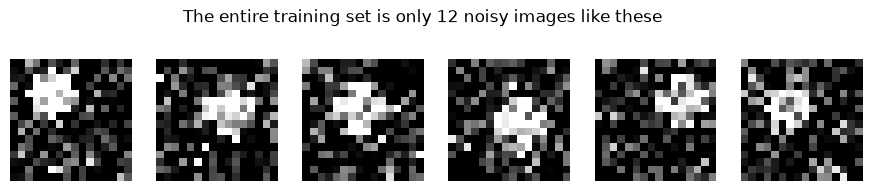
\includegraphics[width=0.85\textwidth]{figures/lesson35_fig01.png}
\caption{The entire training set is only 12 noisy images like these.}
\label{fig:l35-1}
\end{figure}

\section{Watching it overfit}

Train a reasonably large CNN (Chapter~\ref{ch:lesson34}'s architecture) on just these 12 images, and track both training loss and \emph{validation} loss (on the held-out 150 images) at every epoch:

\begin{lstlisting}
for _ in range(epochs):
    loss = F.binary_cross_entropy_with_logits(model(Xtr), ytr)
    loss.backward()
    opt.step()
    val_losses.append(F.binary_cross_entropy_with_logits(model(Xval), yval).item())
\end{lstlisting}

Final train accuracy reaches $100.0\%$, but final validation accuracy is only $72.7\%$; validation loss bottoms out at $0.456$ at epoch 277 (of 400), then climbs back up to $0.573$ by the end (Figure~\ref{fig:l35-2}).

\begin{figure}[h]
\centering
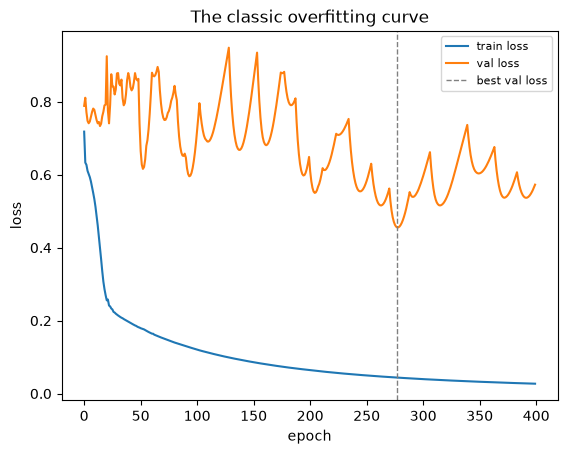
\includegraphics[width=0.6\textwidth]{figures/lesson35_fig02.png}
\caption{The classic overfitting curve: training loss falls monotonically while validation loss bottoms out and rises again.}
\label{fig:l35-2}
\end{figure}

Training loss marches steadily to zero --- the network perfectly memorizes all 12 images, noise included. Validation loss, meanwhile, bottoms out part-way through training and then climbs back up: past that point, every further epoch makes the model \emph{more} confidently wrong about data it hasn't seen. Final validation accuracy lands well short of the training set's perfect score, despite the training set being fit exactly.

\section{Fix 1: data augmentation}

If there isn't enough real data, manufacture more from what's there. Apply random transformations from Chapter~\ref{ch:lesson08} (flips, small rotations) to each training image --- the label doesn't change, but the pixels do, so the network sees a much wider variety of ``what a plus/circle can look like'' instead of memorizing 12 exact images (Figure~\ref{fig:l35-3}). With 20 augmented copies of each of the 12 base images: train accuracy stays at $100.0\%$, but validation accuracy jumps from $72.7\%$ to $95.3\%$.

\begin{figure}[h]
\centering
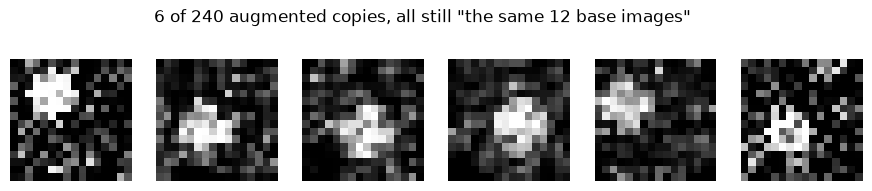
\includegraphics[width=0.85\textwidth]{figures/lesson35_fig03.png}
\caption{6 of 240 augmented copies, all still ``the same 12 base images.''}
\label{fig:l35-3}
\end{figure}

\section{Fix 2: weight decay}

\textbf{Weight decay} adds a penalty proportional to the squared weight magnitudes directly into the loss (equivalently, it shrinks every weight slightly toward zero on every update). Large, highly-tuned weights are exactly what a network needs to memorize 12 specific noisy images; penalizing weight magnitude makes that memorization more costly relative to finding a simpler, smoother function --- without adding a single extra training example. With \code{weight\_decay=0.05}: train accuracy stays at $100.0\%$, validation accuracy rises to $84.0\%$.

\begin{center}
\renewcommand{\arraystretch}{1.3}
\begin{tabular}{lrr}
\hline
\textbf{approach} & \textbf{train acc} & \textbf{val acc} \\
\hline
no fix       & 100.0\% & 72.7\% \\
augmentation & 100.0\% & 95.3\% \\
weight decay & 100.0\% & 84.0\% \\
\hline
\end{tabular}
\end{center}

Both fixes recover a large chunk of the lost validation accuracy, from two different angles: augmentation attacks the problem by giving the model more (synthetic) data to be right about; weight decay attacks it by making the model less willing to contort itself around a small dataset in the first place. In practice, both are normally used together, along with other regularizers like \textbf{dropout}, covered next, and \textbf{batch normalization} (Chapter~\ref{ch:lesson37}), which incidentally also acts as a mild regularizer.

\section{Fix 3: dropout}

\textbf{Dropout} (\citelink{srivastava2014}{Srivastava et al., 2014}) randomly zeroes out a fraction $p$ of a layer's activations on every training step, forcing the surviving units to not rely on any one specific other unit always being present. To keep the layer's output at the same overall scale whether or not dropout is active, the surviving activations are rescaled by $1/(1-p)$ --- this is ``inverted dropout,'' what every framework's \code{Dropout} layer actually implements. At evaluation time, dropout does nothing at all: the full, unmodified layer runs, which is why \code{model.eval()} matters --- forgetting it would leave dropout randomly firing at test time. A from-scratch inverted-dropout implementation zeroes $30.0\%$ of activations against a target $p=0.3$ (PyTorch's \code{F.dropout} zeroes $30.3\%$ on the same seed), and eval-mode dropout is confirmed to be a true no-op.

Applying it to this chapter's overfitting problem needs \emph{some} redundancy to work with --- zeroing half of a 32-unit feature vector going straight into a 1-unit output leaves little room to help, so a wider hidden layer (32 $\to$ 64 $\to$ 1) is added, with dropout on the 64-unit layer. With only 12 training images, results are noisy from one random seed to the next, so mean validation accuracy over 8 seeds is compared rather than a single run: no dropout reaches $62.8\%\pm7.0\%$, dropout($p=0.5$) reaches $70.2\%\pm8.0\%$.

In a toy setting this tiny (just 12 training images), there isn't much redundancy for dropout to exploit yet. Although only a modest improvement is shown here, dropout's benefit is well established at the scale of real datasets and real networks (hundreds of redundant units, thousands of examples). In practice dropout is almost always combined with the other regularizers on this page, not used alone.

\section{Putting it together: real photos, real overfitting}

Every fix so far has been tested one at a time, on a synthetic 12-image toy problem chosen specifically to make the failure mode unmistakable. This closing section repeats the experiment on real \textbf{CIFAR-10} (\citelink{krizhevsky2009cifar}{Krizhevsky, 2009}) photographs: a small, deliberately data-scarce training set of cats and trucks (40 images per class), with augmentation, weight decay, and dropout combined together. Real photographs contain lighting, clutter, and genuine visual ambiguity between classes. Each configuration is averaged over 3 seeds, since 80 training images is still small enough for individual runs to vary:

\begin{center}
\renewcommand{\arraystretch}{1.3}
\begin{tabular}{lrr}
\hline
\textbf{approach} & \textbf{train acc} & \textbf{val acc} \\
\hline
no fix       & 100.0\% & 78.8\% \\
augmentation & 100.0\% & 80.6\% \\
weight decay & 94.6\%  & 75.9\% \\
dropout      & 100.0\% & 77.9\% \\
all combined & 100.0\% & 82.3\% \\
\hline
\end{tabular}
\end{center}

No single fix is a clear winner here. Weight decay alone actually lands \emph{below} the unregularized baseline --- with \code{weight\_decay=0.01}, training accuracy no longer even reaches 100\%, meaning the penalty is strong enough to fight the objective without finding a better solution in its place. That's a useful, humbling result: the \code{weight\_decay=0.05} value used earlier in this chapter was tuned for a much smaller network on 12 tiny synthetic images, and a regularization strength that works well in one setting doesn't automatically transfer to a different architecture or real photographic data.

Augmentation and dropout each recover a modest amount of validation accuracy individually. ``All combined'' beats every single fix and the unregularized baseline, echoing the same lesson from the synthetic dataset: these three regularizers compound rather than substitute for each other. The gain over the unregularized baseline is real but modest (a few percentage points here), which is itself the honest takeaway: regularization narrows the gap between training and validation performance, it doesn't manufacture data or model capacity that isn't there.

Closing that gap further, on real images, takes what later chapters introduce --- more training data, better architectures (Chapter~\ref{ch:lesson37}), and eventually \textbf{transfer learning} (Chapter~\ref{ch:lesson38}): starting from a network already trained on millions of images, instead of memorizing from scratch on a handful of them.

\subsection*{Exercises}
\begin{enumerate}
  \item Try \code{weight\_decay} values of $0.001$, $0.05$, and $1.0$. Is there a point where it starts to \emph{hurt} training accuracy along with (eventually) validation accuracy?
  \item Sweep \code{dropout\_p} over $[0.0, 0.2, 0.4, 0.6, 0.8]$, averaging over the same 8 seeds at each value. Is there a value that's clearly best, or does the mean stay within one standard deviation across most of the range given how little data there is?
  \item Increase the augmentation multiplier from 20 to 100 copies per base image. Does validation accuracy keep improving, or does it plateau --- and if it plateaus, what does that suggest about the fundamental limit of augmenting a dataset that only contains 12 \emph{underlying} examples to begin with?
\end{enumerate}

\vfill
\fullcode{lesson35}{lesson35_training_a_cnn}
